\subsection{ZFS磁盘格式}
\subsubsection{vdev label}
访问文件总是从物理介质的某个已知的固定位置读取文件系统的元数据开始,
传统文件系统的元数据称为超级块,
ZFS的术语就是{\em vdev label}和{\em Uberblock}。
ZFS在磁盘的起始和结尾存储了四份vdev label。
对vdev label的更新是唯一不遵循COW原则的点。
ZFS采用两阶段提交的方法保证完整性,
具体说就是先更新偶数号的label再到奇数号的,
这样万一在更新某个label时发生掉电仍然有健全的label可用。
vdev label的结构及其在磁盘上的分布如图\,\ref{fig:vlabel}\,所示。

\begin{figure}[ht]
  \centering
  \includegraphics[width=\textwidth]{fig/zfs_vdev_label.pdf}
  \caption{Vdev Label}\label{fig:vlabel}
\end{figure}

\subsubsection{块指针}
除位于固定位置的元数据vdev label外,
所有其它数据位置都是动态分配的,
访问它们都必须通过块指针。
确切地说,
块指针是一个数据块的描述子,
除了记载块在磁盘上的逻辑地址以外,
还有较验和,块类型等域,
块指针结构如\,\ref{fig:blkptr}\,所示。

\begin{figure}[ht]
  \centering
  \includegraphics[width=\textwidth]{fig/zfs_blkptr.pdf}
  \caption{Vdev Label}\label{fig:blkptr}
\end{figure}

值得一提的是一个数据块在磁盘上最多可以有三个备份,
ZFS术语称为{\em ditto blocks}。
Uberblock结构有一个\verb|ub_rootbp|域,
游历文件系统数据块就从那里开始。

\subsubsection{对象}
若干数据块以一定方式组织成为对象({\em Object}),
如面向用户的POSIX文件对象(\verb|DMU_OT_PLA-IN_FILE_CONTENTS|)%
和POSIX目录对象(\verb|DMU_OT_DIRECTORY_CONTENTS|),
还有维护ZFS内部逻辑用的\verb|DMU_OT_SPACE_MAP|、
\verb|DMU_OT_DNODE|等对象。

对象的描述子称为{\em dnode},
磁盘上结构为\verb|dnode_phys_t|。
粗略地,
可以把 \verb|dnode_phys_t| 看作 一个模版,
各种类型的对象是这个模版的不同实例,
一个dnode描述相关的数据块如何被组织成该类型的对象。
譬如文件对象描述其所有数据块在磁盘中的分布;
又如目录对象描述如何在该目录下根据文件名检索到对应的文件对象。
dnode类型定义如代码段\,\ref{src:dnode}\,所示。
\inputclisting{zfs_src/dnode.h}
              {ZFS对象}{src:dnode}
一个dnode只包含一个块指针,
ZFS数据块最大尺寸128K,
文件数据超过这一尺寸就需要引入间接块,
ZFS支持最多6级间接寻址,
除第一级间接块尺寸为16K可容纳$2^7$个块指针,
其余均可达到块最大限制128K可容纳$2^{10}$个块指针,
可计算出一个对象的最大尺寸为$2^{7 + 7 + 10 \times 5} = 2^{64}$字节。
图\,\ref{fig:dn_ind}\,演示了一个三级间接寻址。
\begin{figure}[!ht]
  \centering
  \includegraphics[width=.8\textwidth]{fig/zfs_ind_blkptr.pdf}
  \caption{三级间接寻址}\label{fig:dn_ind}
\end{figure}
              
\subsubsection{对象集}
除了负责将数据块组织成对象,
DMU这一层也管理由多个对象组成的对象集({\em Object Set}。)
换句话说是对象集的数据就是一个个dnode。
对象集有三种,
分别是\verb|DMU_OST_META|、\verb|DMU_OST_ZFS|及\verb|DMU_OST_ZVOL|。
磁盘上描述对象集的数据结构{\em objse\_phys\_t}
定义如代码段\,\ref{src:objset}\,。
\newpage
\inputclisting{zfs_src/objset.h}
              {ZFS对象集}{src:objset}

\begin{figure}[!ht]
  \centering
  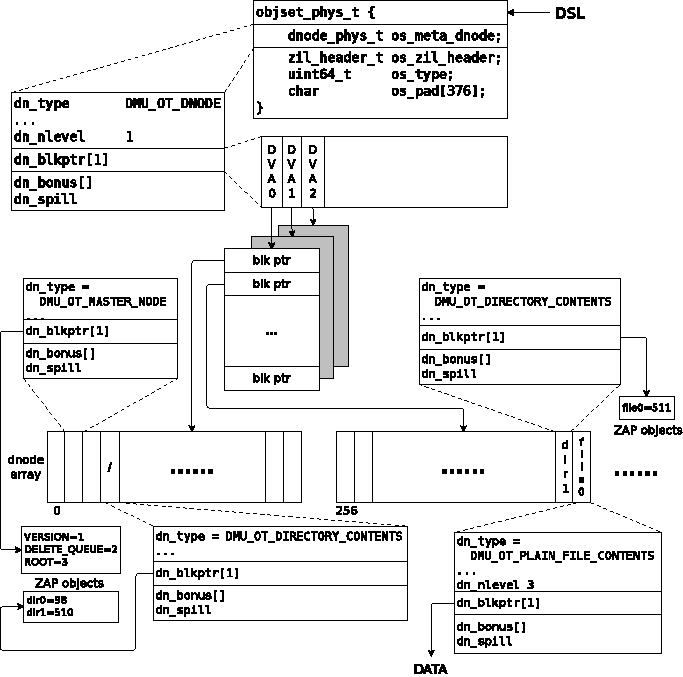
\includegraphics[width=\textwidth]{fig/zfs_objset.pdf}
  \caption{对象集内部组织结构}\label{fig:zfs_objset}
\end{figure}

图\,\ref{fig:zfs_objset}\,示例一个由文件系统对象集定位到指定对象的过程。
从中可以看到,
对象集作为检索对象的起始点,
其结构包含一个dnode类型的域,其类型为\verb|DMU_OT_DNODE|,
换句话说,
该dnode域描述的数据类型为dnode。
另外值得注意的是它的\verb|dn_nlevel|域为1,
说明其描述的dnode寻址树有一级间接寻址。


一个dnode尺寸为512字节,
由上面的计算可知,
一个对象集最多可以容纳$2^{64} / 2^{9} = 2^{55}$个对象。
对象集的数据\,---\,dnode以数组形式存储索引,
每个对象在dnode array中有一个唯一索引号。
索引号为1的dnode有特殊用途,
视对象集的类型而定。
对文件系统类型来说,
该特殊dnode所描述的对象为\verb|DMU_OT_MASTER_NODE|类型,
即一种ZAP对象,
其数据块中存储的信息包括了根目录对象在数组中的索引号,
图中那个``\verb|ROOT=3|''项。
从这里开始就可以遍历访问整个文件系统。
注意到目录类型的对象存储的都是 name-value 对,
value 部分就是对应该名字的dnode在数组中的索引
图中接地的那部分就进入上一节描述的游历一个对象的所有数据块过程。

\subsubsection{DSL}

\begin{figure}[!ht]
  \centering
  \includegraphics[width=.95\textwidth]{fig/zfs_dsl.pdf}
  \caption{MOS dnode数组结构}\label{fig:mos}
\end{figure}

如何检索到到一个指定的对象集由DSL层负责。
DSL层在磁盘上也呈现为一个对象集,
也就是说它所存储处理的数据也是对象描述子\,--dnode,
这一层对象集的类型为\verb|DMU_OST_META|,
即所谓MOS({\em Meta Object Set}),
MOS也是一个dnode数组。
作为目录项,
MOS中很多项的块指针指向的ZAP对象中存储的是另外某些项在数组中索引的位置,
如图\,\ref{fig:mos}\,中的{\em Object Directory}项描述的数据对象中的%
``root dataset=2'',
又如{\em Child Directory}项数据中的%
``myfs=18''。

在刚引入dnode概念的时候有一个细节没有提及,
就是\verb|dn_bonus|域,
该域有时被用来存储比较小的数据避免分配一个大块。
\footnote{{\tt dmu\_bonus\_hold}函数是个好例子。}
例如图\,\ref{fig:mos}\,中,
文件系统dnode为存储管理活跃的数据集的dnode在MOS的索引没有动用块指针那套机制,
而是在\verb|dn_bonus|中存储\verb|dsl_dir_phys_t|的结构,
这个结构的\verb|dd_head_dataset_obj|域就是当前活跃数据集的dnode在MOS中的索引值;
又如描述活跃对象集的dnode的\verb|dn_bonus|域中存储的是%
\verb|dsl_dataset_phys_t|结构,
通过这个结构的\verb|ds_dp|域指向的数据块即可进入由对象集向对象的检索阶段。
无法将下一层的\verb|objset_phys_t|也嵌入到\verb|dn_bonus|中因为%
\verb|objset_phys_t|本身含有一个dnode结构,
不得已只好开一个块来存储它。

MOS如何寻址得到呢?
答案就是Uberblock。
图\,\ref{fig:uber}\,示意如何完成在磁盘上寻址MOS。
如前所述,
vdev label和uberblock作为整个检索树的根,
必须位于磁盘的固定位置为软件层预先知晓。
\begin{figure}[!hb]
  \centering
  \includegraphics[width=.95\textwidth]{fig/zfs_uber_to_mos.pdf}
  \caption{由Uberblock到MOS}\label{fig:uber}
\end{figure}

\subsection{ZFS块管理---{\em Space Map}}
\subsubsection{位图}
传统的块管理一般使用位图,
思路简单,
一个位表示一个块,
一个字节可以表示8个块,
如果采用4K块大小,
在1T的磁盘上,
需要32M字节的位图,
1PB就需要32G字节,
空间使用和扫描位图的时间开销开始不可接受。
为优化扫描效率,
一个看似可行的方案是将位图分区,
每一个区维护一个整数纪录该区的空闲块数量,
这避免了每一次都扫描整个大位图而只需扫描一个小分区,
譬如1PB的大位图可以分成1M个区。
但这方案仍然有个大问题,
不但分配块需要读写位图,
释放块一样需要。
譬如在1PB的文件系统中删除一个4GB的文件,
需要释放1M个块,
也就是说修改1M个位,
如果运气不好,
上述的1M个位图分区都要被访问到,
这开销太大。
另外当内存容纳不下整个位图,
随机地分配和释放块伴随的位图更新操作将导致大量的磁盘写入。

\subsubsection{B-树}
B-树方案就是在磁盘上存储一棵以{\em extent}%
(即一个起始地址和从那开始的长度)为key的B-树,
这解决一个问题,
就是一次分配或释放一个大连续块组,
只做少数的几个磁盘写入即可更新块管理数据结构,
比位图的一一对应效率高了很多。
大量随机分配释放小块使得在树的各个节点都要更新,
也没有大的extent,
都是描述小extent的节点,
巨额开销仍无法避免。

\subsubsection{延迟释放}
对上述两种数据结构可以做一个优化就是延迟释放,
以期未来某个时候需要分配一个新块的时候直接交付,
直到释放块的数量达到一个阈值对要释放的块地址进行排序,
按顺序更新磁盘上的位图或树,
大大降低了开销。

\subsubsection{Space Map}
ZFS则创新地采用类似log结构的方式存储磁盘块使用信息,
称为{\em Space Map}。Jeff Bonwick在他的博客中提到:

\begin{quotation}
  Recall that log-structured filesystems long  ago posed this question: what if,
  instead of periodically folding a transaction log back into the filesystem, we
  made the transaction log be the filesystem?

  Well, the  same question could  be asked of our  deferred free list:  what if,
  instead of folding it into a bitmap  or B-tree, we made the deferred free list
  be the free space representation?
\end{quotation}

ZFS的确就是这么做的。
ZFS把物理设备划分为一百多个slab,
每个slab有一个块管理数据结构 space map,
当分配或释放某个extent时,
就往space map中追加一条log记录下这一事件,
因为它总是以追加方式记录,
并且由于采用了延迟释放,
随机释放和连续释放效率一样,

另外一个美妙的地方在于当加载一个存储池时,
space map会在内存中表现为一棵按磁盘上地址排序的AVL树,
其节点就是所有空闲块的extent。
这样常常可以将多条log抵消,
或合并为一个节点,
使得树并不很大,
在分配和释放过程中AVL也时不时合并和拆分节点,
再将space map写回磁盘去也不会太大。
极端的例子就是加载一个全满和全空的在内存中AVL树结构一样,
就一个节点。
